\subsubsection{Centroid Decomposition (Decomposição em Centróide)}
A Decomposição em Centróide divide recursivamente uma árvore encontrando o
centróide (o nó cuja remoção deixa todas as subárvores com tamanho $\le N/2$).
Isso reduz a altura da árvore de decomposição para $\mathcal{O}(\log N)$, sendo
a ferramenta definitiva para resolver problemas de caminhos e distâncias entre
quaisquer pares de nós na árvore.

Veja a Decomposição em Centróide reduzindo a árvore:\\ \vspace{0.5cm} \noindent
\begin{minipage}[t]{0.31\textwidth}
    \centering
    \textbf{Passo 1: Árvore Original}\\
    \vspace{0.2cm}
    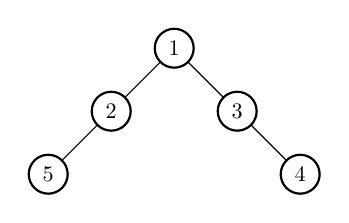
\begin{tikzpicture}[every node/.style={circle, draw, minimum size=0.5cm, thick}, scale=0.8, every node/.append style={transform shape}, >=stealth]
        \node (1) at (0, 1) {1};
        \node (2) at (-1, 0) {2};
        \node (3) at (1, 0) {3};
        \node (4) at (2, -1) {4};
        \node (5) at (-2, -1) {5};
        \draw (1) -- (2);
        \draw (1) -- (3);
        \draw (3) -- (4);
        \draw (2) -- (5);
    \end{tikzpicture}

    \vspace{0.2cm}
    \footnotesize
    \raggedright
    Árvore geral com 5 nós conectados.
\end{minipage}%
\hfill
%
\begin{minipage}[t]{0.31\textwidth}
    \centering
    \textbf{Passo 2: Achar Centróide}\\
    \vspace{0.2cm}
    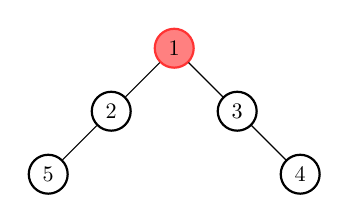
\begin{tikzpicture}[every node/.style={circle, draw, minimum size=0.5cm, thick}, scale=0.8, every node/.append style={transform shape}, >=stealth]
        \node[fill=red!50, draw=red!80] (1) at (0, 1) {1};
        \node (2) at (-1, 0) {2};
        \node (3) at (1, 0) {3};
        \node (4) at (2, -1) {4};
        \node (5) at (-2, -1) {5};
        \draw (1) -- (2);
        \draw (1) -- (3);
        \draw (3) -- (4);
        \draw (2) -- (5);
    \end{tikzpicture}

    \vspace{0.2cm}
    \footnotesize
    \raggedright
    Identifica o nó 1 como centróide (nenhuma subárvore excede $N/2$).
\end{minipage}%
\hfill
%
\begin{minipage}[t]{0.31\textwidth}
    \centering
    \textbf{Passo 3: Árvore de Centróides}\\
    \vspace{0.2cm}
    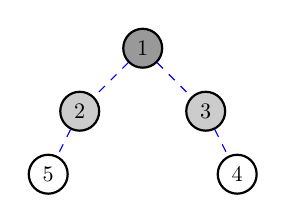
\begin{tikzpicture}[every node/.style={circle, draw, minimum size=0.5cm, thick}, scale=0.8, every node/.append style={transform shape}, >=stealth]
        \node[fill=gray!80] (1) at (0, 1) {1};
        \node[fill=gray!40] (2) at (-1, 0) {2};
        \node[fill=gray!40] (3) at (1, 0) {3};
        \node (4) at (1.5, -1) {4};
        \node (5) at (-1.5, -1) {5};
        \draw[dashed, blue] (1) -- (2);
        \draw[dashed, blue] (1) -- (3);
        \draw[dashed, blue] (3) -- (4);
        \draw[dashed, blue] (2) -- (5);
    \end{tikzpicture}

    \vspace{0.2cm}
    \footnotesize
    \raggedright
    Remove o centróide e repete recursivamente, formando a árvore de centróides (altura $\le \log N$).
\end{minipage}

\vspace{0.3cm}

\paragraph{Implementação: }\mbox{}\\
\textbf{C++:}
\begin{lstlisting}[language=C++]
vector<vector<int>> adj;
vector<bool> removed;
vector<int> sub_size;

void get_sub_size(int u, int p) {
    sub_size[u] = 1;
    for (int v : adj[u]) {
        if (v != p && !removed[v]) {
            get_sub_size(v, u);
            sub_size[u] += sub_size[v];
        }
    }
}

int get_centroid(int u, int p, int total) {
    for (int v : adj[u]) {
        if (v != p && !removed[v] && sub_size[v] > total / 2)
            return get_centroid(v, u, total);
    }
    return u;
}

void decompose(int u) {
    get_sub_size(u, u);
    int centroid = get_centroid(u, u, sub_size[u]);
    
    removed[centroid] = true;
    
    // Processa o centroide atual (ex: caminhos que passam por ele)
    
    for (int v : adj[centroid]) {
        if (!removed[v]) decompose(v);
    }
}
\end{lstlisting}